%%%%%%%%%%%%%%%%%%%%%%%%%%%%%%%%%%%%%%%%%%%%%%%%%%%%%%%%%%%%%%%%%%%%%%
% How to use writeLaTeX: 
%
% You edit the source code here on the left, and the preview on the
% right shows you the result within a few seconds.
%
% Bookmark this page and share the URL with your co-authors. They can
% edit at the same time!
%
% You can upload figures, bibliographies, custom classes and
% styles using the files menu.
%
%%%%%%%%%%%%%%%%%%%%%%%%%%%%%%%%%%%%%%%%%%%%%%%%%%%%%%%%%%%%%%%%%%%%%%

\documentclass[12pt]{article}
\usepackage{adjustbox}
\usepackage{sbc-template}
\usepackage{todonotes}
\usepackage{graphicx,url}
\usepackage{amsmath}
\usepackage{multirow}
\usepackage[utf8]{inputenc}  
\usepackage[T1]{fontenc}
\usepackage{xspace}
\usepackage{url}
\usepackage{graphicx}
\usepackage{subfig}
%----------
\usepackage{unicode-math}
\usepackage{babel}
\babeltags{br = brazil, en = english}
%\setmathfont{xits-math.otf}
\usepackage{listings}
\usepackage[]{algorithm2e}
%\setmathfont[math-style=upright,range={`e,`i}]{xits-math.otf}
% Definindo novas cores
\usepackage{xcolor}
\definecolor{verde}{rgb}{0.25,0.5,0.35}
\definecolor{jpurple}{rgb}{0.5,0,0.35}
\definecolor{darkgreen}{rgb}{0.0, 0.2, 0.13}
\newcommand{\estiloR}{
  \lstset{ %
    language=R,                     % the language of the code
    basicstyle=\footnotesize,       % the size of the fonts that are used for the code
    numbers=left,                   % where to put the line-numbers
    numberstyle=\tiny\color{gray},  % the style that is used for the line-numbers
    stepnumber=1,                   % the step between two line-numbers. If it's 1, each line
                                    % will be numbered
    numbersep=5pt,                  % how far the line-numbers are from the code
    backgroundcolor=\color{white},  % choose the background color. You must add \usepackage{color}
    showspaces=false,               % show spaces adding particular underscores
    showstringspaces=false,         % underline spaces within strings
    showtabs=false,                 % show tabs within strings adding particular underscores
    frame=single,                   % adds a frame around the code
    rulecolor=\color{black},        % if not set, the frame-color may be changed on line-breaks within not-black text (e.g. commens (green here))
    tabsize=2,                      % sets default tabsize to 2 spaces
    captionpos=b,                   % sets the caption-position to bottom
    breaklines=true,                % sets automatic line breaking
    breakatwhitespace=false,        % sets if automatic breaks should only happen at whitespace
    title=\lstname,                 % show the filename of files included with \lstinputlisting;
                                    % also try caption instead of title
    keywordstyle=\color{blue},      % keyword style
    commentstyle=\color{darkgreen},   % comment style
    stringstyle=\color{red},      % string literal style
    escapeinside={\%*}{*)},         % if you want to add a comment within your code
    morekeywords={*,...}          % if you want to add more keywords to the set
}}


%--------------
\sloppy

\title{Sistemas Operacionais\\Produtor/Consumidor}


\author{Prof. Dr. Gerson Cavalheiro \inst{1},\\Guilherme de Souza\inst{1}}

\begin{document} 

\maketitle
\br
\section{Execução}
Para este trabalho foi fornecido um \textit{Makefile} junto ao código, para facilitar a sua execução. Com isso basta executar o comando:

\textbf{make}\\
Logo após para executar o programa deve-se utilizar o seguinte comando seguido dos parâmetros esperado por ele:

\textbf{./producer\_consumer <num\_it><num\_prod><num\_cons><tam\_buffer>}
\begin{itemize}
    \item\textbf{num\_it}: Número de iterações passado para os produtores.
    \item\textbf{num\_prod}: Número de produtores.
    \item\textbf{num\_cons}: Número de consumidores.
    \item\textbf{tam\_buffer}: Tamanho maximo do buffer.
\end{itemize}

\section{Relatório}

Para implementação deste trabalho, parti da leitura da teoria/funcionabilidade do produtor/consumidor. O que não foi uma tarefa complicada, fazer-se entender foi o passo mais simples. Em seguida para que a implementação do mesmo fosse possivel, o conhecimento de pthreds se fez necessario (como pedido pelo trabalho, dado que não poderia fazer uso do threads do C++ 11).

Em um primeiro momento realizei a implementação de um pseudo código com o que eu realmente gostaria de programar.

\begin{algorithm}[H]
\caption{Pseudo código para o produtor}
	\KwData{numero\_iteracoes, tamanho\_buffer}
	%\KwResult{void}
		\While{\Delta i < numero\_iteracoes}{
            \If{buffer == numero\_iteracoes}{
              espera até mudar\;
            }
			
            secao\_critica\;
            buffer.push(rand())\;
            fim\_secao\_critica\;
            %$\Delta i \leftarrow N^2$ \;
			%\eIf{$V_f$ \neq $S_i$}{
			%	atualizaOsValores\;
			%	$N \leftarrow V_f$ + 2\;
			}%{
			%	$N \leftarrow S_i$ - 7\;
			%}
			
			%$N \leftarrow N + 1$ \;
		}
\end{algorithm}


\begin{algorithm}[H]
\caption{Pseudo código para o consumidor}
	%\KwData{}
	%\KwResult{void}
		\While{true}{
            \If{buffer == vazio}{
              espera até mudar\;
            }
			
            secao\_critica\;
            \If{buffer.front() == -1}{
                buffer.pop()\;
                break\;
            }
            
            e\_primo(buffer.front())\;

            \If{e\_primo}{
                imprime(thread\_id : numero\_tirado\_do\_buffer)
            }
            
            buffer.pop()\;
            fim\_secao\_critica\;
            %$\Delta i \leftarrow N^2$ \;
			%\eIf{$V_f$ \neq $S_i$}{
			%	atualizaOsValores\;
			%	$N \leftarrow V_f$ + 2\;
			}%{
			%	$N \leftarrow S_i$ - 7\;
			%}
			
			%$N \leftarrow N + 1$ \;
		}
\end{algorithm}

Partindo do pseudo código pude ver alguns erros como: lugar onde seria necessario a seção critica e como a lista devia se comportar para que ela seguisse o padrão FIFO. Para solucionar a parte da lista, bastou fazer uso correto das funções ja dadas pelo \textit{list} do C++ 11, inserindo atrás e removendo na frente.

Quanto a seção critica, para um melhor aproveitamento, fez-se uso de variaveis locais, que são visiveis somente ao escopo da função. Dessa forma pude paralelizar a parte de verificar se um numero é primo ou não e a parte de imprimir os que são dados como primos. 

Para realizar o que era necessario algumas funções espesíficas foram necesárias: 
\begin{itemize}
    \item \textbf{pthread\_cond\_await()}: dessa forma conseguia esperar o sinal de que havia algo no buffer, ou que tinha espaço para inserir mais itens. Dessa forma colocava a thread em espera de forma correta, conseguindo fazer a liberação do mutex, assim não deixando ninguem presso a espera dele.
    \item \textbf{pthred\_cond\_signal()}: para que as threads em espera pudessem sair do seu estado de \textit{sleep}, toda vez que era terminado de inserir e remover um item do buffer, um sinal era mandado. Dessa forma tenho um controle maior sobre o que esta acontecendo com o buffer.
    \item \textbf{pthread\_mutex\_lock()} e \textbf{pthread\_mutex\_unlock()}: assim conseguia criar a seção critica tanto para ver se estava cheio ou vazio o buffer, como para inserir ou remover o item do mesmo. Assim evitando os problemas comum do produtor/consumidor, que é inserir tendo um item no local, ou consumir nem um item, ou até duas ou mais \textit{threads} consumirem o mesmo.    
\end{itemize}

Enquanto o código estava em contrução pude observar alguns pontos, como o uso correto das funções da biblioteca e observar os pontos onde realmente é necessário uma seção critica ou não. parece meio obvio falando assim, mas uma programação mais no \textit{"hardcoding"} mostra que o desempenho melhora e muito. 

Porém dado o número de iterações pequeno para um determinado numero de \textit{threads}, a eficiência não é demonstrada. Dado o custo de criação de uma \textit{thread} e sua execução. Agora quando o numero de iterações é grande suficiênte, é possivel ver ganhos reais.

\section{hardware usado}

Para obtenção das infromações sobre o \textit{hardware} usado para algumas execuções, usou-se o comando \textbf{lscpu}, como pode ser visto abaixo: 

\begin{scriptsize}
\estiloR
\begin{lstlisting}[caption={informações CPU}, label=lst:rcode]
Architecture:        x86_64
CPU op-mode(s):      32-bit, 64-bit
Byte Order:          Little Endian
Address sizes:       36 bits physical, 48 bits virtual
CPU(s):              4
On-line CPU(s) list: 0-3
Thread(s) per core:  2
Core(s) per socket:  2
Socket(s):           1
NUMA node(s):        1
Vendor ID:           GenuineIntel
CPU family:          6
Model:               58
Model name:          Intel(R) Core(TM) i5-3230M CPU @ 2.60GHz
Stepping:            9
CPU MHz:             1197.298
CPU max MHz:         3200.0000
CPU min MHz:         1200.0000
BogoMIPS:            5188.11
Virtualization:      VT-x
L1d cache:           32K
L1i cache:           32K
L2 cache:            256K
L3 cache:            3072K
NUMA node0 CPU(s):   0-3
\end{lstlisting}
\end{scriptsize}

\section{Visualização usando HTOP}

De forma que fosse possivel visualizar as \textit{threads} criadas e, se de fato estava em funcionamento (partindo é claro do que o \textit{hardware} nos possibilita), algumas execuções foram realizadas usando o \textbf{htop} como ferramenta de visualização. 

Em um primeiro momento executou-se número pequenos de iterações e \texit{threads}, porém a visualização nem era percebivel de fato (algo sobre já foi comentado em seções anteriores). Com isso partimos de execuções com números grandes. Primeiro podemos visualizar o uso da máquina na figura 1 antes da execução do código.

\begin{figure}[ht]
\centering
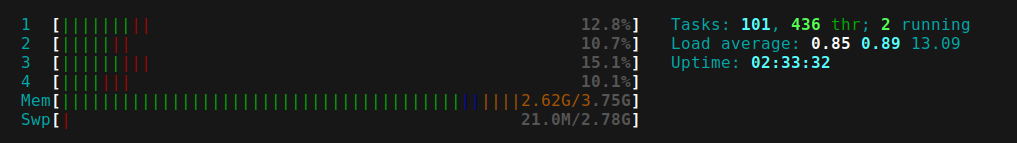
\includegraphics[width=1\textwidth]{/home/souza//Documents/antes_certo.png}}
\caption{Visualização htop antes da execução do código}
\label{fig:exampleFig1}
\end{figure}

Com isso executou-se o código com os seguintes parâmetros demonstrados na tabela 1. Usou-se um tamanho de buffer pequeno, para desta forma fosse possivel ver \textit{threads} paradas, com isso a visualização no htop se torna melhor. Mas denovo dado o limite da máquina os valores não crescem tanto, pela administração do próprio sistema perante as \textit{threads} exigidas ou umfato não averiguado no momento. Mas é possivel ver que a máquina encontra-se com 100\% de uso, como demonstra a figura 2 e o numero de \textit{threads} cresce também.

\begin{table}[!h]
\centering
\begin{tabular}{l|c}
\multicolumn{1}{c|}{\textbf{Parâmetros}} & \multicolumn{1}{l}{\textbf{Valores}} \\ \hline
Número de iterações                      & 10000                                \\ \hline
Número de Produtores                     & 500                                  \\ \hline
Número de Consumidores                   & 500                                  \\ \hline
Tamanho do buffer                        & 100                                  \\ \hline
\end{tabular}
    \caption{Tabela com parâmetros passados para primeira execução do código}
\end{table}

\begin{figure}[!h]
\centering
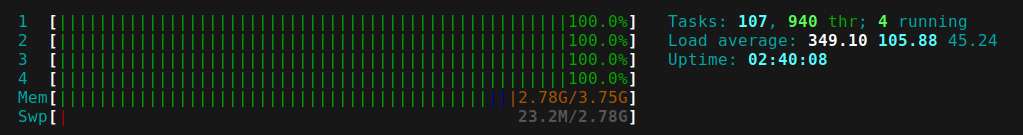
\includegraphics[width=1\textwidth]{/home/souza//Documents/primeira.png}}
\caption{Visualização via htop durante execução do código}
\end{figure}

Com isso, aumentou-se o numero de \textit{threads} em uso, para ver se esse "up" seria visivel via htop. Segui os mesmos passo anterior, podendo obervar os parâmetros na tabela 2 e o número de \textit{threads} antes e depois da execução do código na figura 3 e 4 respectivamente.


\begin{table}[!h]
\centering
\begin{tabular}{l|c}
\multicolumn{1}{c|}{\textbf{Parâmetros}} & \multicolumn{1}{l}{\textbf{Valores}} \\ \hline
Número de iterações                      & 10000                                \\ \hline
Número de Produtores                     & 1000                                  \\ \hline
Número de Consumidores                   & 1000                                 \\ \hline
Tamanho do buffer                        & 100                                  \\ \hline
\end{tabular}
    \caption{Tabela com parâmetros passados para segunda execução do código}
\end{table}

\begin{figure}[!h]
\centering
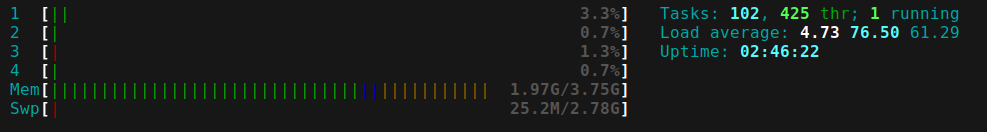
\includegraphics[width=1\textwidth]{/home/souza//Documents/antes_certo_2.png}}
\caption{Visualização via htop antes da execução do código}
\end{figure}

\begin{figure}[!h]
\centering
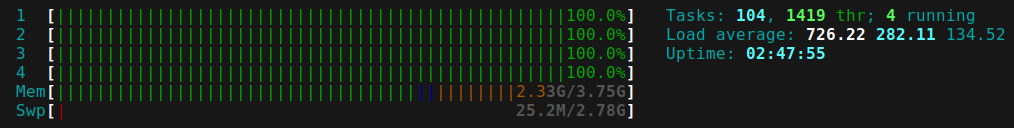
\includegraphics[width=1\textwidth]{/home/souza//Documents/segunda_execucao_resultado.png}}
\caption{Visualização via htop durante execução do código}
\end{figure}

Através das figuras, tornou-se possivel observar que o número de \textit{threads} se manteve quase sempre pela metade do que era pedido, possivelmente dado o \textit{hardware} em uso e, o próprio controle do sistema como ja comentado. Revisão no código foram feitas e comparações com de colegas para encontrar possíveis erros, porém, nada foi visivel, logo fica meu questionamento.

\end{document}
